% CSE 276A HW2 report: closed-loop waypoint driving with AprilTag landmarks.
% Compile with pdflatex (e.g. upload this folder to Overleaf). Figures are in figures/,
% every number below comes from data/ (see README.md for where each one is).
\documentclass[10pt]{article}
\usepackage[margin=0.8in]{geometry}
\usepackage{amsmath}
\usepackage{graphicx}
\usepackage{booktabs}
\usepackage{tikz}
\usetikzlibrary{arrows.meta,positioning,calc}
\usepackage{hyperref}
\usepackage{enumitem}
\setlist{nosep}
\setlength{\parskip}{3pt}
\setlength{\parindent}{0pt}

\title{\vspace{-1.5em}HW2: Closed-Loop Waypoint Driving with AprilTags}
\author{Soham Lokhande \quad CSE 276A}
\date{November 2026}

\begin{document}
\maketitle
\vspace{-1.5em}

\textbf{Video:} \url{https://youtu.be/TODO} \qquad
\textbf{Route:} $(0,0,0)\to(1,0,0)\to(1,2,\pi)\to(0,0,0)$ (m, rad), option 1 (AprilTags).

\section*{Coordinate frames and start pose}
\begin{itemize}
  \item \textbf{World:} origin at the start mark, $+x$ toward waypoint $(1,0)$, $+y$ to the left, $\theta$ counter-clockwise from $+x$.
  \item \textbf{Vehicle:} origin at the turning centre (middle of the wheels), $x$ forward, $y$ left. This point is the one placed on the floor marks.
  \item \textbf{Sensor (camera):} optical frame of the IMX219 camera, $x$ right, $y$ down, $z$ forward. The lens sits $d = 0.10$\,m ahead of the turning centre.
  \item \textbf{Tag:} AprilTag frame with $z$ pointing out of the printed face, toward the viewer.
  \item \textbf{Start pose:} $(0, 0, 0)$, turning centre on the start mark, facing $+x$.
\end{itemize}

\section*{(a) Closed-loop controller}
\begin{center}
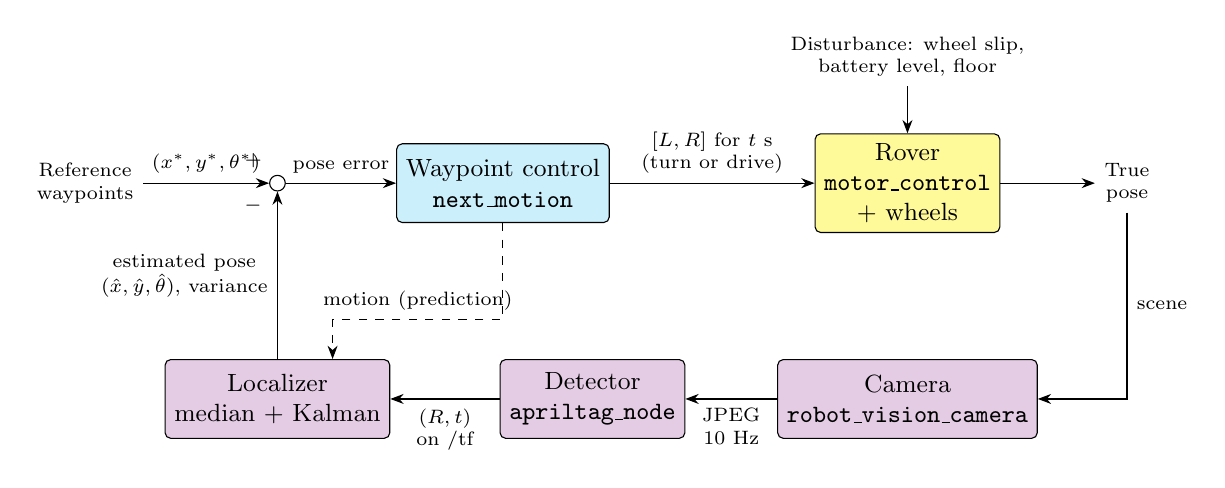
\begin{tikzpicture}[>=Stealth, node distance=8mm and 12mm,
    blk/.style={draw, rounded corners=2pt, align=center, minimum height=10mm, font=\small},
    lbl/.style={font=\scriptsize, align=center}]
  \node[circle, draw, inner sep=2pt] (sum) {};
  \node[left=16mm of sum, lbl] (ref) {Reference\\waypoints};
  \node[blk, fill=cyan!20, right=14mm of sum] (ctrl) {Waypoint control\\\texttt{next\_motion}};
  \node[blk, fill=yellow!40, right=26mm of ctrl] (sys) {Rover\\\texttt{motor\_control}\\+ wheels};
  \node[right=12mm of sys, lbl] (out) {True\\pose};
  \node[blk, fill=violet!20, below=16mm of sys] (cam) {Camera\\\texttt{robot\_vision\_camera}};
  \node[blk, fill=violet!20] (loc) at (sum |- cam) {Localizer\\median + Kalman};
  \node[blk, fill=violet!20] (tag) at ($(loc)!0.5!(cam)$) {Detector\\\texttt{apriltag\_node}};
  \node[above=6mm of sys, lbl] (dist) {Disturbance: wheel slip,\\battery level, floor};
  \draw[->] (ref) -- node[above, lbl] {$(x^*, y^*, \theta^*)$} (sum);
  \node[lbl, above left=0mm and 0mm of sum] {$+$};
  \node[lbl, below left=0mm and 0mm of sum] {$-$};
  \draw[->] (sum) -- node[above, lbl] {pose error} (ctrl);
  \draw[->] (ctrl) -- node[above, lbl] {$[L,R]$ for $t$ s\\(turn or drive)} (sys);
  \draw[->] (dist) -- (sys);
  \draw[->] (sys) -- (out);
  \draw[->] (out) |- node[pos=0.25, right, lbl] {scene} (cam);
  \draw[->] (cam) -- node[below, lbl] {JPEG\\10 Hz} (tag);
  \draw[->] (tag) -- node[below, lbl] {$(R, t)$\\on /tf} (loc);
  \draw[->] (loc) -- node[left, lbl] {estimated pose\\$(\hat x, \hat y, \hat\theta)$, variance} (sum);
  \draw[->, dashed] (ctrl.south) |- node[pos=0.75, above, lbl] {motion (prediction)} ([xshift=7mm, yshift=5mm]loc.north) -- ([xshift=7mm]loc.north);
\end{tikzpicture}
\end{center}

The robot drives \emph{stop-and-go}: it stops, looks at the tags, decides, and moves; the loop closes once per stop.
\begin{itemize}
  \item \textbf{Camera} (\texttt{robot\_vision\_camera}): IMX219 at $1280\times720$, 10 Hz, rectified with our calibration; publishes the image (JPEG) and \texttt{camera\_info}.
  \item \textbf{Detector} (\texttt{apriltag\_node}): finds tag36h11 tags (14.35 cm) and publishes each tag's pose $(R, t)$ in the camera frame on \texttt{/tf}.
  \item \textbf{Localizer} (in \texttt{closed\_loop\_follower}): keeps the pose estimate and its variance. Each motion predicts the new pose (unicycle model); each stop corrects it with the tag sightings (part (c)).
  \item \textbf{Waypoint control} (\texttt{next\_motion}): compares the estimate with the current waypoint. Within 5 cm the waypoint is reached; within 15 cm it only drives forward/back; otherwise it turns toward the waypoint if more than $5^\circ$ off, else drives 25 cm (or the whole rest if under 40 cm). At a reached waypoint it turns to the waypoint heading.
  \item \textbf{Rover control} (\texttt{motor\_control}): sends the wheel command $[L, R]$ at 20 Hz over serial to the motor board for the computed time. Times come from our HW1 calibration: drive 0.263 m/s; turn $77.5^\circ$/s left and $99.1^\circ$/s right, plus a start-up delay.
\end{itemize}

\section*{(b) Landmarks}
\begin{center}
\small
\begin{tabular}{cccl}
\toprule
Tag & Position (m) & Faces & Used on \\
\midrule
1 & $(1.4, 0.0)$ & $-x$ & leg 1 toward $(1,0)$; final heading check at $(0,0)$ \\
2 & $(1.0, 2.4)$ & $-y$ & leg 2 toward $(1,2)$ \\
0 & $(-0.4, 0.0)$ & $+x$ & leg 3 toward $(0,0)$ \\
\bottomrule
\end{tabular}
\end{center}
Each tag stands 0.4 m \emph{past} a waypoint on the line of the leg that ends there, at camera height, facing the approaching robot. The reasons:
\begin{itemize}
  \item The robot faces its next waypoint on almost every stop, so the tag is near the image centre, where detection and pose are most accurate.
  \item The tag is never closer than about 0.4 m, so it never leaves the $64^\circ\times38^\circ$ field of view or fills the whole frame.
  \item It gets closer as the robot nears the waypoint, so the fixes are most accurate exactly where the waypoint error is measured. Pose noise grows with range.
\end{itemize}
Known gaps: at $(1,2)$ facing $\pi$ no tag is in view, so that heading is dead reckoning. Tag 0 is at an angle to leg 3, so it leaves the view in the last $\sim$40 cm of the leg.

\section*{(c) Pose estimation and noise}
\textbf{From one sighting to a pose.} \texttt{apriltag\_node} gives the tag's translation $t$ and rotation $R$ in the camera frame. In the vehicle frame, the tag is at forward $f = t_z + d$ and left $l = -t_x$. The tag's face normal is the third column of $R$, so its direction seen from the robot is $\alpha = \operatorname{atan2}(-R_{02}, R_{22})$ ($\alpha \approx \pi$ when facing it squarely). With the tag's known map position $(x_T, y_T)$ and facing $\varphi$:
\[
\theta_{\text{meas}} = \varphi - \alpha, \qquad
\begin{pmatrix} x \\ y \end{pmatrix}_{\text{meas}} =
\begin{pmatrix} x_T \\ y_T \end{pmatrix} -
\begin{pmatrix} \cos\hat\theta & -\sin\hat\theta \\ \sin\hat\theta & \cos\hat\theta \end{pmatrix}
\begin{pmatrix} f \\ l \end{pmatrix}.
\]

\textbf{Handling the noise.}
\begin{enumerate}
  \item \emph{Stand still to measure.} Images are taken only after a 1 s settle, so there is no motion blur and no timing mismatch between the image and the pose.
  \item \emph{Median over frames.} Each stop collects 0.8 s of sightings (7--9 frames). The per-tag median removes single-frame outliers such as PnP orientation flips; a tag seen in fewer than 2 frames is ignored.
  \item \emph{Kalman filter.} The filter keeps a variance for position ($P_{xy}$) and heading ($P_\theta$).
    \begin{itemize}
      \item Each motion adds noise: 5\% of a drive's length, and 6\% of a turn's angle plus $1^\circ$.
      \item Measurement noise grows with the range $r$: $\sigma_\theta = 2^\circ + 3^\circ/\text{m}\cdot r$ and $\sigma_{xy} = 1\,\text{cm} + 2\,\text{cm/m}\cdot r$.
      \item Each update is $\hat s \leftarrow \hat s + k(s_{\text{meas}} - \hat s)$ with $k = P/(P+\sigma^2)$.
      \item Heading is fused first, and the position measurement uses the fused heading. A tag's orientation is its noisiest output, and multiplying it by the range would move the position.
    \end{itemize}
  \item \emph{Outlier gate.} A sighting more than $3\sigma$ from the prediction (and at least $30^\circ$ or 0.40 m away) is rejected. Because the gate widens with the prediction's variance, a correct tag is still accepted after a long stretch without one.
\end{enumerate}
\textbf{Why this design.} Our motors are open-loop and HW1 showed turns repeat only to about $\pm5^\circ$. The camera is accurate when the robot stands still near a tag: 1.02 m measured at a taped 1.00 m. Weighting the two by their variances lets each tag fix pull the estimate back, without one bad frame throwing it off. In practice the gate caught a real error: in an earlier run tag 2 had been placed 1 m from its map position, and every sighting of it was rejected.

\section*{(d) No landmark in view}
The robot \textbf{never drives unless the stop right before the drive saw a tag}. Turning to a waypoint heading is allowed without a tag.

If a stop sees no tag, the robot \textbf{searches}:
\begin{enumerate}
  \item It uses the map to find the tags that should be visible from its estimated pose (range, viewing angle, printed side), and turns toward the nearest-in-angle one, trying up to two such tags.
  \item If that fails, it sweeps in $40^\circ$ steps (less than the $64^\circ$ field of view, so there are no gaps), looking after each step.
  \item After a fix it turns back toward the waypoint and continues. A full circle without a tag stops the run with an error rather than driving blind.
\end{enumerate}
Between fixes the pose comes from the motion model, and its growing variance widens the gate for the next sighting.

This happened once in the run: 59 cm before $(0,0)$, tag 0 left the view. One map-guided search turn of $-32^\circ$ found it, the robot turned back $+31^\circ$ and finished the leg.

\section*{(f) Smoothness}
The motion is deliberately \emph{not} smooth: 23 drives and 9 turns, each followed by a 1.0 s settle and a 0.8 s look.
\begin{itemize}
  \item Of the 89.5 s run, the wheels turned for only 28.4 s.
  \item Each 25 cm drive is a short, nearly constant-speed segment (0.95 s at 0.263 m/s). The fixed commands are the ones calibrated in HW1, so every motion is repeatable.
  \item The camera corrections between stops were small: 2.8 cm and $0.9^\circ$ on average, at most 9.8 cm and $2.4^\circ$. So the path stays close to the straight reference lines (figure in (i)) instead of zig-zagging.
\end{itemize}
The cost is speed; a continuous controller with tag fixes while moving would be smoother but would have to handle motion blur and the image delay.

\section*{(g) Total moving distance}
\begin{center}
\small
\begin{tabular}{lccc}
\toprule
 & Leg 1 & Leg 2 & Leg 3 \\
\midrule
Driven (m) & 1.19 & 2.16 & 2.39 \\
\bottomrule
\end{tabular}
\end{center}
\textbf{Total: 5.73 m = 11.5 units of 0.5 m, plus $451^\circ$ (7.9 rad) of rotation}, in 89.5 s.

The reference path is 5.24 m long and needs $360^\circ$ of turning. The extra comes from:
\begin{itemize}
  \item the forward/back corrections near the waypoints;
  \item four small heading corrections ($\pm6^\circ$);
  \item the $\pm32^\circ$ search turn on leg 3.
\end{itemize}

\section*{(h) Error at each waypoint}
\begin{center}
\small
\begin{tabular}{lccc}
\toprule
Waypoint & Position reached (estimate) & Translation error & Rotation error \\
\midrule
$(1, 0, 0)$     & $(0.964, 0.088, -1.5^\circ)$ & 9.6 cm & $1.5^\circ$ \\
$(1, 2, \pi)$   & $(0.957, 1.981, 180.0^\circ)$ & 4.7 cm & $0.0^\circ$\,$^\dagger$ \\
$(0, 0, 0)$     & $(0.017, 0.031, -2.0^\circ)$ & 3.5 cm & $2.0^\circ$ \\
\bottomrule
\end{tabular}
\end{center}
Errors are from the robot's localizer, at the moment it declared each waypoint reached.
% TODO: replace with tape measurements of the turning centre against the floor marks if taken.
$^\dagger$No tag is visible facing $\pi$ at $(1,2)$, so this heading is dead reckoning after a fix $99^\circ$ earlier; the true error is likely a few degrees (turns repeat to about $\pm5^\circ$).

At $(1,0)$ most of the error is sideways (8.8 cm). Within 15 cm of a waypoint the controller only drives forward/back, because a few centimetres to the side is a large angle at that range and turning there caused oscillation in earlier runs. So the sideways offset left after the leg is kept.

\section*{(i) 2D trajectory}
\begin{center}
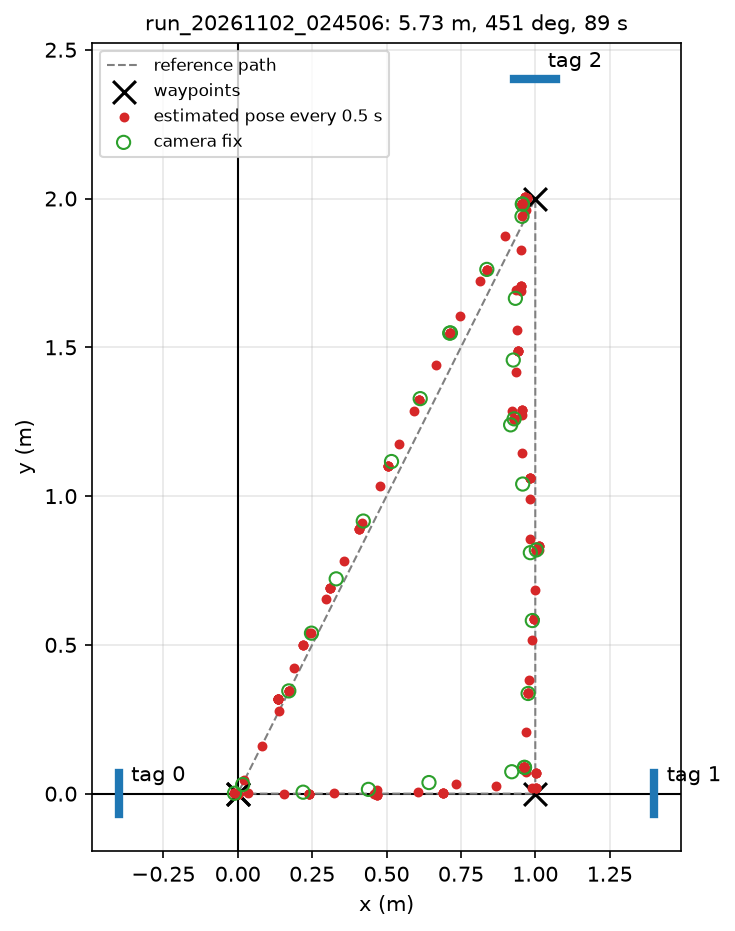
\includegraphics[width=0.48\linewidth]{figures/trajectory.png}
\end{center}
\vspace{-0.5em}
Red dots: the robot's own pose estimate every 0.5 s (prediction while moving, Kalman estimate while stopped). Green circles: stops with a tag fix (30 of 34 stops). Grey dashed: reference path. Blue bars: tags, drawn along the printed face.

\section*{(j) Reflection}
\textbf{What worked.} The final run reached all three waypoints within 10 cm by the robot's own estimate, with 30 of 34 stops getting a tag fix and no rejected readings. Placing each tag behind its waypoint meant the robot almost always looked straight at a tag, and the per-stop corrections stayed under 10 cm.

\textbf{What went wrong on the way}, and what we learned:
\begin{enumerate}
  \item The original OV5647 camera module was dead on I2C; we replaced it with an IMX219.
  \item Only 1--3 of the 10 raw 2.7 MB images per second reached the detector. We switched the detector to the camera's compressed stream, which arrived at the full 10 Hz.
  \item Turn rates dropped by half on a low battery. We now calibrate and run on a full charge.
  \item A search bug measured every turn from the starting heading.
  \item A tag placed 1 m from its map position. The outlier gate correctly rejected every one of its sightings, but this left the robot searching instead of driving.
\end{enumerate}
Most of the debugging time went into the sensing pipeline, not the controller.

\textbf{Limitations and next steps.}
\begin{itemize}
  \item \emph{Sideways error.} The 15 cm approach rule cannot remove a sideways offset (8.8 cm at $(1,0)$). A short turn-drive-turn manoeuvre at 15--30 cm would fix it.
  \item \emph{Noisy heading at range.} A tag's orientation is noisy beyond $\sim$2 m. Using its bearing, $\operatorname{atan2}(l, f)$, together with its known position would give a steadier heading.
  \item \emph{Blind heading at $(1,2,\pi)$.} A fourth tag near $(0.4, 2.0)$ facing $+x$ would cover it.
  \item \emph{Unmeasured offset.} The lens offset $d$ was estimated, not measured.
  \item \emph{Speed.} Stop-and-go is slow (68\% of the time standing still). Fusing fixes while moving at low speed would be the next step for smoothness.
\end{itemize}

\section*{Code}
ROS 2 Jazzy workspace (\url{https://github.com/lokhandesoham/CSE276Robot}, branch \texttt{main}):
\begin{itemize}
  \item \texttt{robot\_control}: \texttt{closed\_loop\_follower.py} (stop-and-go loop, search), \texttt{localization.py} (sighting geometry, Kalman filter, map), \texttt{calibration.py} (HW1 motion model), \texttt{motor\_control}.
  \item \texttt{robot\_vision}: the camera node and our camera calibration (\texttt{camera\_parameter.yaml}).
  \item \texttt{apriltag\_ros}: the detector with our tag configuration (\texttt{tags\_36h11.yaml}).
  \item \texttt{landmarks.txt}, \texttt{waypoints\_hw2.txt}: the map and the route.
\end{itemize}
\end{document}
